\documentclass[a4paper,12pt]{article}

% ====== PACKAGES ======
\usepackage[utf8]{inputenc}
\usepackage[T1]{fontenc}
\usepackage{lmodern}
\usepackage[english]{babel}
\usepackage{amsmath, amssymb}
\usepackage{siunitx}
\usepackage{graphicx}
\usepackage{float}
\usepackage{caption}
\usepackage{subcaption}
\usepackage{booktabs}
\usepackage{geometry}
\usepackage[hidelinks]{hyperref}
\usepackage{tikz}
\usetikzlibrary{shapes,arrows,positioning}
\geometry{margin=1in}

% ====== TITLE ======
\title{System Performance - Bit Error Rate Calculation}
\author{Wannes Baes}

% ====== DOCUMENT ======
\begin{document}


\maketitle
\vspace{-1em} % reduces space after title

\noindent This document presents the calculations of a theoretical upper bound and approximation for the bit error rate (BER) of the single-user multi-input multi-output (SU-MIMO) singular value decomposition (SVD) communication system.




\begin{figure}[H]
\centering

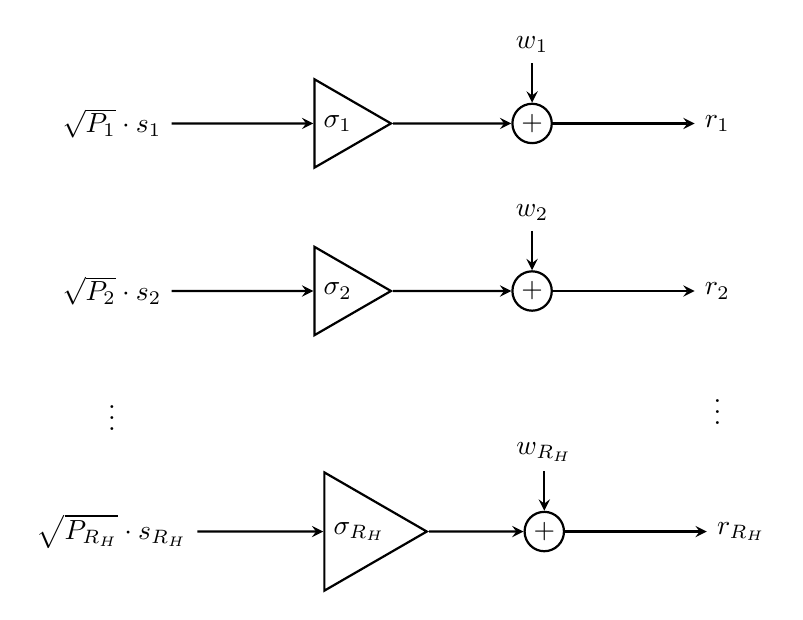
\begin{tikzpicture}[node distance=2cm, auto, thick, >=stealth]

    % Define block styles
    \tikzstyle{triangle} = [draw, isosceles triangle, isosceles triangle apex angle=60, minimum width=1cm, minimum height=0.5cm]
    \tikzstyle{sum} = [draw, circle, inner sep=1pt, minimum size=0.5cm, node distance=2cm]
    \tikzstyle{signal} = [coordinate]

    % Row 1
    \node (s1) {$\sqrt{P_1} \cdot s_1$};
    \node[triangle, right=1.8cm of s1] (sigma1) {$\sigma_1$};
    \node[sum, right=1.5cm of sigma1] (sum1) {+};
    \node[right=1.8cm of sum1] (r1) {$r_1$};
    \node[above=0.5cm of sum1] (w1) {$w_1$};

    \draw[->] (s1) -- (sigma1);
    \draw[->] (sigma1) -- (sum1);
    \draw[->] (sum1) -- (r1);
    \draw[->] (w1) -- (sum1);

    % Row 2
    \node[below=1.5cm of s1] (s2) {$\sqrt{P_2} \cdot s_2$};
    \node[triangle, right=1.8cm of s2] (sigma2) {$\sigma_2$};
    \node[sum, right=1.5cm of sigma2] (sum2) {+};
    \node[right=1.8cm of sum2] (r2) {$r_2$};
    \node[above=0.5cm of sum2] (w2) {$w_2$};

    \draw[->] (s2) -- (sigma2);
    \draw[->] (sigma2) -- (sum2);
    \draw[->] (sum2) -- (r2);
    \draw[->] (w2) -- (sum2);

    % Dotted ellipsis line
    \node[below=0.8cm of s2] (dots_s) {$\vdots$};
    \node[below=0.8cm of r2] (dots_r) {$\vdots$};

    % Row R_H
    \node[below=0.8cm of dots_s] (sN) {$\sqrt{P_{R_H}} \cdot s_{R_H}$};
    \node[triangle, right=1.6cm of sN] (sigmaN) {$\sigma_{R_H}$};
    \node[sum, right=1.2cm of sigmaN] (sumN) {+};
    \node[right=1.8cm of sumN] (rN) {$r_{R_H}$};
    \node[above=0.5cm of sumN] (wN) {$w_{R_H}$};

    \draw[->] (sN) -- (sigmaN);
    \draw[->] (sigmaN) -- (sumN);
    \draw[->] (sumN) -- (rN);
    \draw[->] (wN) -- (sumN);

\end{tikzpicture}

\caption{The $R_H$ parallel eigenchannels of the decomposed SU-MIMO SVD system.}
\end{figure}
\bigskip

\noindent The BER of the complete SU-MIMO SVD system can be computed as the weighted average of the BERs of each eigenchannel of the system.

\begin{equation}
\mathrm{BER} = \frac{1}{C_{\text{total}}} \sum_{i=0}^{R_{H}} \left\lfloor C_i \right\rfloor \mathrm{BER}_i
\end{equation}

\noindent The total used capacity of the system equals the sum of the used capacities of each eigenchannel: $ C_{\text{total}} = \sum_{i=0}^{R_{H}} \left\lfloor C_i \right\rfloor $

\paragraph{Capacity of the eigenchannels.}
The capacity of each eigenchannel $C_i$ can be computed using the Shannon capacity formula.

\begin{equation}
    C_i = 2B \cdot \log_2(1 + \frac{P_i \sigma^{2}_i}{2B N_0}) \label{eq:Ci}
\end{equation}
\paragraph{Bit Error Rate of the eigenchannels \cite{syllabus_communicatietheorie}.}
The BER of each eigenchannel $\mathrm{BER}_i$ equals the average amount of bit errors per received data symbol.

\begin{equation}
    \mathrm{BER}_i = \frac{1}{\log_2{M_i}} \sum_{(\hat{\alpha}, \alpha) \in \mathcal{C}^{2}_i} \mathrm{N}(\hat{\alpha}, \alpha) \cdot \mathrm{P}[\hat{s}_i = \hat{\alpha} \land s_i = \alpha] \label{eq:BERi}
\end{equation}

\noindent In the above equation:
\begin{itemize}

    \item $ M_i $ is the size of the modulation constellation used in eigenchannel $i$.

    \item $ \mathcal{C}^{2}_i $ is the Cartesian product of the modulation constellation used in eigenchannel $i$ with itself, representing all possible pairs of transmitted and received symbols.
    
    \item $ \mathrm{N}(\hat{\alpha}, \alpha) $ is the number of bit errors between symbol $\alpha$ and symbol $\hat{\alpha}$. This equals the Hamming distance between the binary representations of both symbols.

    \item $ \mathrm{P}[\hat{s}_i = \hat{\alpha} \land s_i = \alpha] $ is the joint probability that symbol $\alpha$ was transmitted and symbol $\hat{\alpha}$ was detected in eigenchannel $i$.

\end{itemize}

\noindent We can simplify this expression using Bayes' rule and by assuming that all symbols are equally likely to be transmitted. The latter is the case when the bits that arrive at the transmitter are independent and equally distributed.

\begin{align}
    \mathrm{BER}_i &= \frac{1}{\log_2{M_i}} \sum_{(\hat{\alpha}, \alpha) \in \mathcal{C}^{2}_i} \mathrm{N}(\hat{\alpha}, \alpha) \cdot \mathrm{P}[\hat{s}_i = \hat{\alpha} \mid s_i = \alpha] \cdot \mathrm{P}[s_i = \alpha] \notag \\
    \mathrm{BER}_i &= \frac{1}{\log_2{M_i}} \sum_{(\hat{\alpha}, \alpha) \in \mathcal{C}^{2}_i} \mathrm{N}(\hat{\alpha}, \alpha) \cdot \mathrm{P}[\hat{s}_i = \hat{\alpha} \mid s_i = \alpha] \cdot \frac{1}{M_i} \notag \\
    \mathrm{BER}_i &= \frac{1}{M_i \log_2{M_i}} \sum_{(\hat{\alpha}, \alpha) \in \mathcal{C}^{2}_i} \mathrm{N}(\hat{\alpha}, \alpha) \cdot \mathrm{P}(\hat{\alpha}, \alpha) \label{eq:BERi-derivation}
\end{align}
\bigskip


\section{Upper Bound}

At the receiver, the symbol $ \hat{\alpha} $ will be detected iff the distance between the decision variable $ u_i $ and $ \hat{\alpha} $ is less than the distance between $ u_i $ and any other symbol in the constellation. In other words, $ u_i $ needs to lie within the decision area $ D(\hat{\alpha}) $ of the symbol $ \hat{\alpha} $.

\begin{equation}
    \mathrm{P}(\hat{\alpha}, \alpha) = \mathrm{P}(u_i \in D(\hat{\alpha}) \mid s_i = \alpha) \label{eq:decision-probability}
\end{equation}

\medskip
\noindent The decision variable $ u_i $ is given by the output of the equalizer at the receiver.

\begin{align}
    u_i &= \frac{1}{\sigma_i \sqrt{P_i}} \cdot r_i  \notag \\
    u_i &= \frac{1}{\sigma_i \sqrt{P_i}} \cdot (\sigma_i \sqrt{P_i} \cdot s_i + n_i)  \notag \\
    u_i &= s_i + \frac{1}{\sigma_i \sqrt{P_i}} n_i  \notag \\
    u_i &= s_i + n'_i \label{eq:decision-variable}
\end{align}

\noindent in which $ \vec{n} = \mathrm{U}^{H} \vec{w} $ is the noise vector after the unitary transformation at the receiver, which does not change the distribution of the noise. Therefore, the noise term $ n'_i $ is complex, circularly symmetric Gaussian distributed with $ n'_i \sim \mathcal{CN}(0, \frac{N_0}{P_i \sigma^{2}_i}) $. 

\noindent So we find that the decision variable $ u_i $ is a complex, circularly symmetric Gaussian random variable with mean $ s_i $ and variance $ \frac{N_0}{P_i \sigma^{2}_i} $.

\paragraph{The upper bound:}
\begin{equation}
    \mathrm{P}(\hat{\alpha}, \alpha) \leq \mathrm{P}\Big( |u_i - \hat{\alpha}| < |u_i - \alpha| \;\big|\; s_i = \alpha \Big) \label{eq:upper-bound}
\end{equation}
It is a necessary condition for $ u_i $ to be closer to $ \hat{\alpha} $ than to $ \alpha $ in the complex plane in order to be detected as $\hat{\alpha}$.
It is however not a sufficient condition, since yet another symbol in the constellation could be even closer to $ u_i $ than $ \hat{\alpha} $. \smallskip

\noindent This is why the above expression is an upper bound. It can be interpreted as the probability that the noise $ n'_i $ causes the decision variable $ u_i $ to cross the decision boundary that lies halfway between $ \alpha $ and $ \hat{\alpha} $, instead of the probability that $ n'_i $ causes $ u_i $ to enter the  decision area of $ \hat{\alpha} $. \bigskip

\noindent We simplify the right hand side of \autoref{eq:upper-bound}.

\begin{align}
    &= \mathrm{P}\Big( |u_i - \hat{\alpha}|^2 < |u_i - \alpha|^2 \;\big|\; s_i = \alpha \Big) \notag \\
    &= \mathrm{P}\Big( |u_i - \alpha - (\hat{\alpha} - \alpha)|^2 < |u_i - \alpha|^2 \;\big|\; s_i = \alpha \Big) \notag \\
    &= \mathrm{P}\Big( |u_i - \alpha - (\hat{\alpha} - \alpha)|^2 - |u_i - \alpha|^2 < 0 \;\big|\; s_i = \alpha \Big) \notag \\
    &= \mathrm{P}\Big( |\hat{\alpha} - \alpha|^2 - 2 \Re \big((u_i - \alpha) (\hat{\alpha} - \alpha)^*\big) < 0 \;\big|\; s_i = \alpha \Big) \notag \\
    &= \mathrm{P}\Big( \Re \big((u_i - \alpha)  (\hat{\alpha} - \alpha)^*\big) > \frac{|\hat{\alpha} - \alpha|^2}{2} \;\big|\; s_i = \alpha \Big) \notag \\
    &= \mathrm{P}\Big( \Re \big((u_i - \alpha) \frac{(\hat{\alpha} - \alpha)^*}{|\hat{\alpha} - \alpha|}\big) > \frac{|\hat{\alpha} - \alpha|}{2} \;\big|\; s_i = \alpha \Big) \notag \\
    &= \mathrm{P}\Big( \Re \big((u_i - \alpha) e^{j \theta} \big) > \frac{|\hat{\alpha} - \alpha|}{2} \;\big|\; s_i = \alpha \Big) \notag \\
    &= \mathrm{Q} \Big(  \frac{|\hat{\alpha} - \alpha|}{2} \cdot \frac{1}{\frac{N_0}{2 P_i \sigma^{2}_i}} \Big) \notag \\
    &= \mathrm{Q} \Big(  \frac{P_i \sigma^{2}_i}{N_0} \cdot |\hat{\alpha} - \alpha| \Big) \label{eq:simplified-upper-bound}
\end{align}

\noindent In the penultimate step, we used the fact that $ \mathrm{X} = \Re \big((u_i - \alpha) e^{j \theta} \big) \;\big|\; (s_i = \alpha) $ is a real-valued Gaussian random variable with mean $ 0 $ and variance $ \sigma = \frac{N_0}{2 P_i \sigma^{2}_i} $. \smallskip

\noindent This can be seen from the fact that $ u_i - \alpha | (s_i = \alpha) = u_i - s_i = n'_i $. The noise term $ n'_i $ is circularly symmetric complex Gaussian, so rotation by $ e^{j \theta} $ does not change its distribution, and the real component is normally distributed with the same mean and half the variance. \bigskip

\noindent Thus, with this upper bound on $ \mathrm{P}(\hat{\alpha}, \alpha) $ and using \autoref{eq:BERi-derivation}, we can compute an upper bound on the BER of each eigenchannel $ \mathrm{BER}_i $ as follows

\begin{equation}
    \mathrm{BER}_i \leq \frac{1}{M_i \log_2{M_i}} \sum_{(\hat{\alpha}, \alpha) \in \mathcal{C}^{2}_i} \mathrm{N}(\hat{\alpha}, \alpha) \cdot \mathrm{Q} \Big(  \frac{P_i \sigma^{2}_i}{N_0} \cdot |\hat{\alpha} - \alpha| \Big) \label{eq:BERi-upper-bound}
\end{equation}


\section{Approximation}

We only consider symbol errors for which the decision variable $ u_i $ is converted to one of the nearest neighbors of the transmitted symbol $ s_i = \alpha $. 
In other words, we only take into account the terms in the summation of \autoref{eq:BERi-upper-bound} (or \autoref{eq:BERi-derivation}) for which $ \hat{\alpha} $ is a nearest neighbor of $ \alpha $ in the modulation constellation. \smallskip

\noindent In this way, we can derive an accurate approximation for the BER of each eigenchannel, starting from \autoref{eq:BERi-upper-bound}.

\begin{equation}
    \mathrm{BER}_i \approx \frac{1}{M_i \log_2{M_i}} \sum_{\alpha \in \mathcal{C}_i} \sum_{\hat{\alpha} \in \mathcal{S(\alpha)}} \mathrm{N}(\hat{\alpha}, \alpha) \cdot \mathrm{Q} \Big(  \frac{P_i \sigma^{2}_i}{N_0} \ d_{\text{min}} \Big)
\end{equation}

\noindent In the above equation:
\begin{itemize}

    \item $ \mathcal{S(\alpha)} $ is the set of nearest neighbors of symbol $\alpha$ in the modulation constellation.
    
    \item $ d_{min} $ is the minimum distance between two symbols in the modulation constellation. This is a constant for a given constellation type and size.

\end{itemize}

\noindent Because we make use of gray coding during the mapping of bits to symbols, the Hamming distance $ \mathrm{N}(\hat{\alpha}, \alpha) $ between two nearest neighbor symbols equals 1 for all pairs of nearest neighbors.

\begin{align}
    \mathrm{BER}_i &\approx \frac{1}{M_i \log_2{M_i}} \sum_{\alpha \in \mathcal{C}_i} \sum_{\hat{\alpha} \in \mathcal{S(\alpha)}} \mathrm{Q} \Big(  \frac{P_i \sigma^{2}_i}{N_0}  d_{\text{min}} \Big) \notag \\
    \mathrm{BER}_i &\approx \frac{1}{\log_2{M_i}}  \mathrm{Q} \Big(  \frac{P_i \sigma^{2}_i}{N_0}  d_{\text{min}} \Big) \cdot \frac{1}{M_i} \sum_{\alpha \in \mathcal{C}_i} \big| \mathcal{S(\alpha)} \big| \label{eq:BERi-approximation-with-sum}
\end{align}

\noindent The last term in \autoref{eq:BERi-approximation-with-sum} represents the average number of nearest neighbors per symbol in the constellation. This equals a constant $ K $ that only depends on the type and size of used constellation. \smallskip

\noindent Therefore, we can further simplify \autoref{eq:BERi-approximation-with-sum} to obtain a final approximation for the BER of each eigenchannel.

\begin{equation}
    \mathrm{BER}_i \approx \frac{K}{\log_2{M_i}}  \mathrm{Q} \Big(  \frac{P_i \sigma^{2}_i}{N_0}  d_{\text{min}} \Big) \label{eq:BERi-approximation} 
\end{equation}
\bigskip

\noindent The constants $ K $ and $ d_{\min} $ can easily be calculated for the modulation constellations that are considered in this system. \autoref{table:K-and-dmin-values} provides the formulas.

\begin{table}[H]
\centering
\renewcommand{\arraystretch}{1.5}
\begin{tabular}{lcc}
    \toprule
    \text{Constellation} & \textbf{$K$}                                         & \textbf{$d_{\min}$}                   \\
    \midrule
    $M$-PAM             & $\dfrac{2(M - 1)}{M}$                                 & $\sqrt{\dfrac{12}{M^2 - 1}}$          \\
    $M$-PSK             & $\begin{cases}1, & M = 2 \\ 2, & M > 2 \end{cases}$   & $2 \cdot | \sin( \frac{\pi}{M}) |$    \\
    $M$-QAM             & $\dfrac{4(\sqrt{M} - 1)}{\sqrt{M}}$                   & $\sqrt{\dfrac{6}{M - 1}}$             \\
    \bottomrule
\end{tabular}
\caption{The average number of nearest neighbors $ K $ and the distance between nearest neighbors $ d_{\min} $ for common constellations.}
\label{table:K-and-dmin-values}
\end{table}

% ====== BIBLIOGRAPHY ======
\bibliographystyle{ieeetr}
\bibliography{references}


\end{document}